\documentclass[a4paper,14pt]{article} % формат документа

\usepackage{cmap} % поиск в ПДФ
\usepackage[T2A]{fontenc} % кодировка
\usepackage[utf8]{inputenc} % кодировка исходного текста
\usepackage[english,russian]{babel} % локализация и переносы
\usepackage[left = 2cm, right = 1cm, top = 2cm, bottom = 2 cm]{geometry} % поля
\usepackage{listings}
\usepackage{float}
\usepackage{graphicx} % для вставки рисунков
\usepackage{amsmath}
\usepackage[table,xcdraw]{xcolor}
\graphicspath{{pictures/}}
\DeclareGraphicsExtensions{.pdf,.png,.jpg}
\newcommand{\anonsection}[1]{\section*{#1}\addcontentsline{toc}{section}{#1}}

\lstset{ %
	language=Python,                % Язык программирования 
	numbers=left,                   % С какой стороны нумеровать          
	frame=single,                    % Добавить рамку
}

\begin{document}
	\begin{titlepage}

       		\begin{center}
         		\large
		
        			Государственное образовательное учреждение высшего профессионального образования\\
       			“Московский государственный технический университет имени Н.Э.Баумана”
         		\vspace{3cm}
            
            		\textsc{Дисциплина: Анализ алгоритмов}
           		\vspace{0.5cm}
                
            		\textsc{Лабораторная работа № 7}
           		 \vspace{3cm}
            
           		 \LARGE 
		 
		 	Алгоритмы сравнения с образцом
           		 \vspace{3cm}
            
            		\begin{flushright}
            			Студент: \\
				Сиденко Анастасия Генадьевна \\   
            			Группа: ИУ7-53Б \\
           			\hfill
            
           			Преподаватели: \\
				Строганов Юрий Владимирович \\
           			Волкова Лилия Леонидовна
            			\vfill
            		\end{flushright}
		
			\large
            		2019 г.
		\end{center}

	\end{titlepage}
    
	\tableofcontents
	
	\newpage
    
	\anonsection{Введение}
	\hfill
	
	Те, кому приходиться часто работать с текстовыми редакторами, часто пользуются функцией нахождения нужных слов в тексте, которая существенно облегчает редактирование документов и поиск нужной информации.
	
	Действительно, современные программы обработки текста включают в свой функционал поиск и замену текстовых фрагментов[1].
	
	Конечно, сейчас функции поиска входят во многие языки программирования высокого уровня – чтобы найти строчку в небольшом тексте используется встроенная функция[2]. 
	
	\hfill
	
	\textbf{Цель} данной работы изучить и разработать алгоритм поиска подстроки в строке. 
	
	\textbf{Задачи данной работы. }
	\begin{enumerate}
	\item Изучить основные алгоритмы, решающих задачу поиска. 
	\item Реализовать данные алгоритмы. 
	\end{enumerate}

	\newpage


        \section{Аналитическая часть}
        \hfill

        Необходимо изучить алгоритмы поиска подстроки в строке. 

        \subsection{Описание задачи}
        \hfill
        
        Поиск строки формально определяется следующим образом. Пусть задан массив $S$ элементов и массив $X$ элементов. Поиск строки обнаруживает первое вхождение $X$ в $S$, результатом будем считать индекс $i$, указывающий на первое с начала строки (с начала массива $S$) совпадение со словом.
        
        \subsection{Пути решения}
        \begin{enumerate}
        \item \textbf{Алгоритм Кнута-Морриса-Пратта}
        
        Алгоритм был разработан Кнутом и Праттом и независимо от них Моррисом в 1977 г.
        
        После частичного совпадения начальной части подстроки $X$ с соответствующими символами строки $S$ мы фактически знаем пройденную часть строки и может «вычислить» некоторые сведения (на основе самого подстроки $X$), с помощью которых потом быстро продвинемся по тексту.
        
        Идея КМП-поиска -- при каждом несовпадении двух символов текста и образа образ сдвигается на самое длинное совпадение начала с концом префикса (не учитывая тривиальное совпадение самого с собой) [3].
        
        \textbf{Пример. }
        
        Создается массив сдвигов, таблица 1. 
        
        \begin{center}
	\begin{tabular}{|c|c|c|l|l|l|}
	\hline
	0 & 1 & 2 & 3 & 4 & 5 \\ \hline
	a & b & c & a & b & d \\ \hline
	0 & 0 & 0 & 1 & 2 & 0 \\ \hline
	\end{tabular}
	
	Таблица 1.
	Массив сдвигов.  
	\end{center}
	
        В таблице 2 представлена работа алгоритма. 	

        \begin{center}
	\begin{tabular}{|l|l|l|l|l|l|l|l|l|l|l|l|l|l|l|l|}
	\hline
	cтрока    & a & b & c & a & b & e                         & a & b & c & a                         & b                         & c                         & a                         	& b                         & d                         \\ \hline
	подстрока & a & b & c & a & b & \cellcolor[HTML]{FE0000}d &   &   &   &                           &                           &                           	&                           &                           &                           \\ \hline
	подстрока &   &   &   & a & b & \cellcolor[HTML]{FE0000}c & a & b & d &                           &                           &                           	&                           &                           &                           \\ \hline
	подстрока &   &   &   &   &   & \cellcolor[HTML]{FE0000}a & b & c & a & b                         & d                         &                           	&                           &                           &                           \\ \hline
	подстрока &   &   &   &   &   &                           & a & b & c & a                         & b                         & \cellcolor[HTML]{FE0000}d &                           &                           &                           \\ \hline
	подстрока &   &   &   &   &   &                           &   &   &   & \cellcolor[HTML]{34FF34}a & \cellcolor[HTML]{34FF34}b & 	\cellcolor[HTML]{34FF34}c & \cellcolor[HTML]{34FF34}a & \cellcolor[HTML]{34FF34}b & \cellcolor[HTML]{34FF34}d 	\\ \hline
	\end{tabular}
	
	Таблица 2.
	Алгоритм КМП.  
	\end{center}
        
        
        \item \textbf{Алгоритм Бойера-Мура}
        
        Алгоритм поиска строки Бойера -- Мура считается наиболее быстрым среди алгоритмов общего назначения, предназначенных для поиска подстроки в строке. Был разработан Бойером и Муром в 1977 году. Преимущество этого алгоритма в том, что ценой некоторого количества предварительных вычислений над шаблоном (но не над строкой, в которой ведётся поиск) шаблон сравнивается с исходным текстом не во всех позициях -- часть проверок пропускаются как заведомо не дающие результата.
        
        Основная идея алгоритм -- начать поиск не с начала, а с конца подстроки. Наткнувшись на несовпадение, мы просто смещаем подстроку до самого правого вхождения данного символа, не учитывая последний [3].
        
        
          \textbf{Пример. }
        
        Создается массив прыжков, таблица 3. 
        
        \begin{center}
	\begin{tabular}{|c|c|c|l|l|l|}
	\hline
	a & b & c & a & b & d \\ \hline
	2 & 1 & 3 & 2 & 1 & 6 \\ \hline
	\end{tabular}
	
	Таблица 3.
	Массив прыжков.  
	\end{center}
	
        В таблице 4 представлена работа алгоритма. 	

        \begin{center}
	\begin{tabular}{|l|l|l|l|l|l|l|l|l|l|l|l|l|l|l|l|}
	\hline
	cтрока    & a & b & c & a & b & e                         & a & b & c & a                         & b                         & c                         & a                         	& b                         & d                         \\ \hline
	подстрока & a & b & c & a & b & \cellcolor[HTML]{FE0000}d &   &   &   &                           &                           &                           	&                           &                           &                           \\ \hline
	подстрока &   &   &   &   &   &                           & a & b & c & a                         & b                         & \cellcolor[HTML]{FE0000}d &                           &                           &                           \\ \hline
	подстрока &   &   &   &   &   &                           &   &   &   & \cellcolor[HTML]{34FF34}a & \cellcolor[HTML]{34FF34}b & 	\cellcolor[HTML]{34FF34}c & \cellcolor[HTML]{34FF34}a & \cellcolor[HTML]{34FF34}b & \cellcolor[HTML]{34FF34}d 	\\ \hline
	\end{tabular}
	
	Таблица 4.
	Алгоритм БМ.  
	\end{center}

        \end{enumerate}
        	                
        \subsection{Выводы} 
        \hfill
        
        В данной работе стоит задача реализации алгоритмов поиска подстроки в строке. 


	\newpage

	\section{Конструкторская часть}
	\hfill

		
	\subsection{Функциональная модель}
	
	На рисунке 1 представлена функциональная модель нашей задачи.  
	
	\begin{center}
		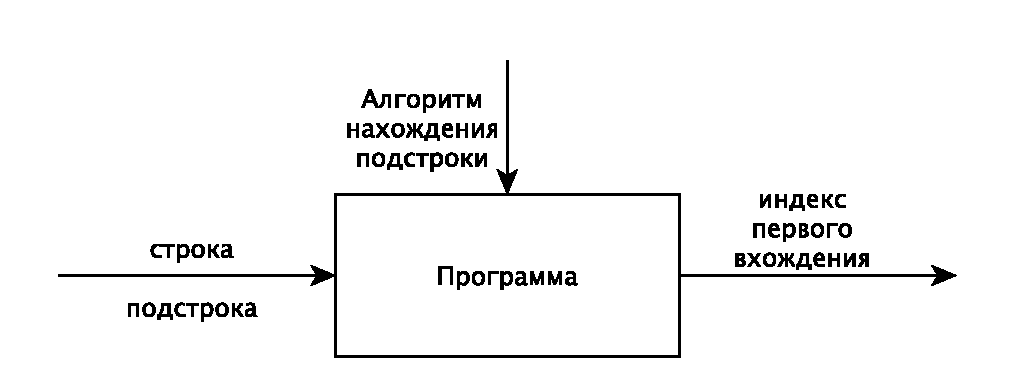
\includegraphics[scale = 0.8]{idef0} \\ Рис.  1 - Функциональная модель алгоритма нахождения вхождения подстроки в строку 
	\end{center}
	        
        \subsection{Схемы алгоритмов}
        \hfill
        
         Приведем схемы алгоритмов (см. рисунки 2 и 3). 
	
	\begin{center}
        		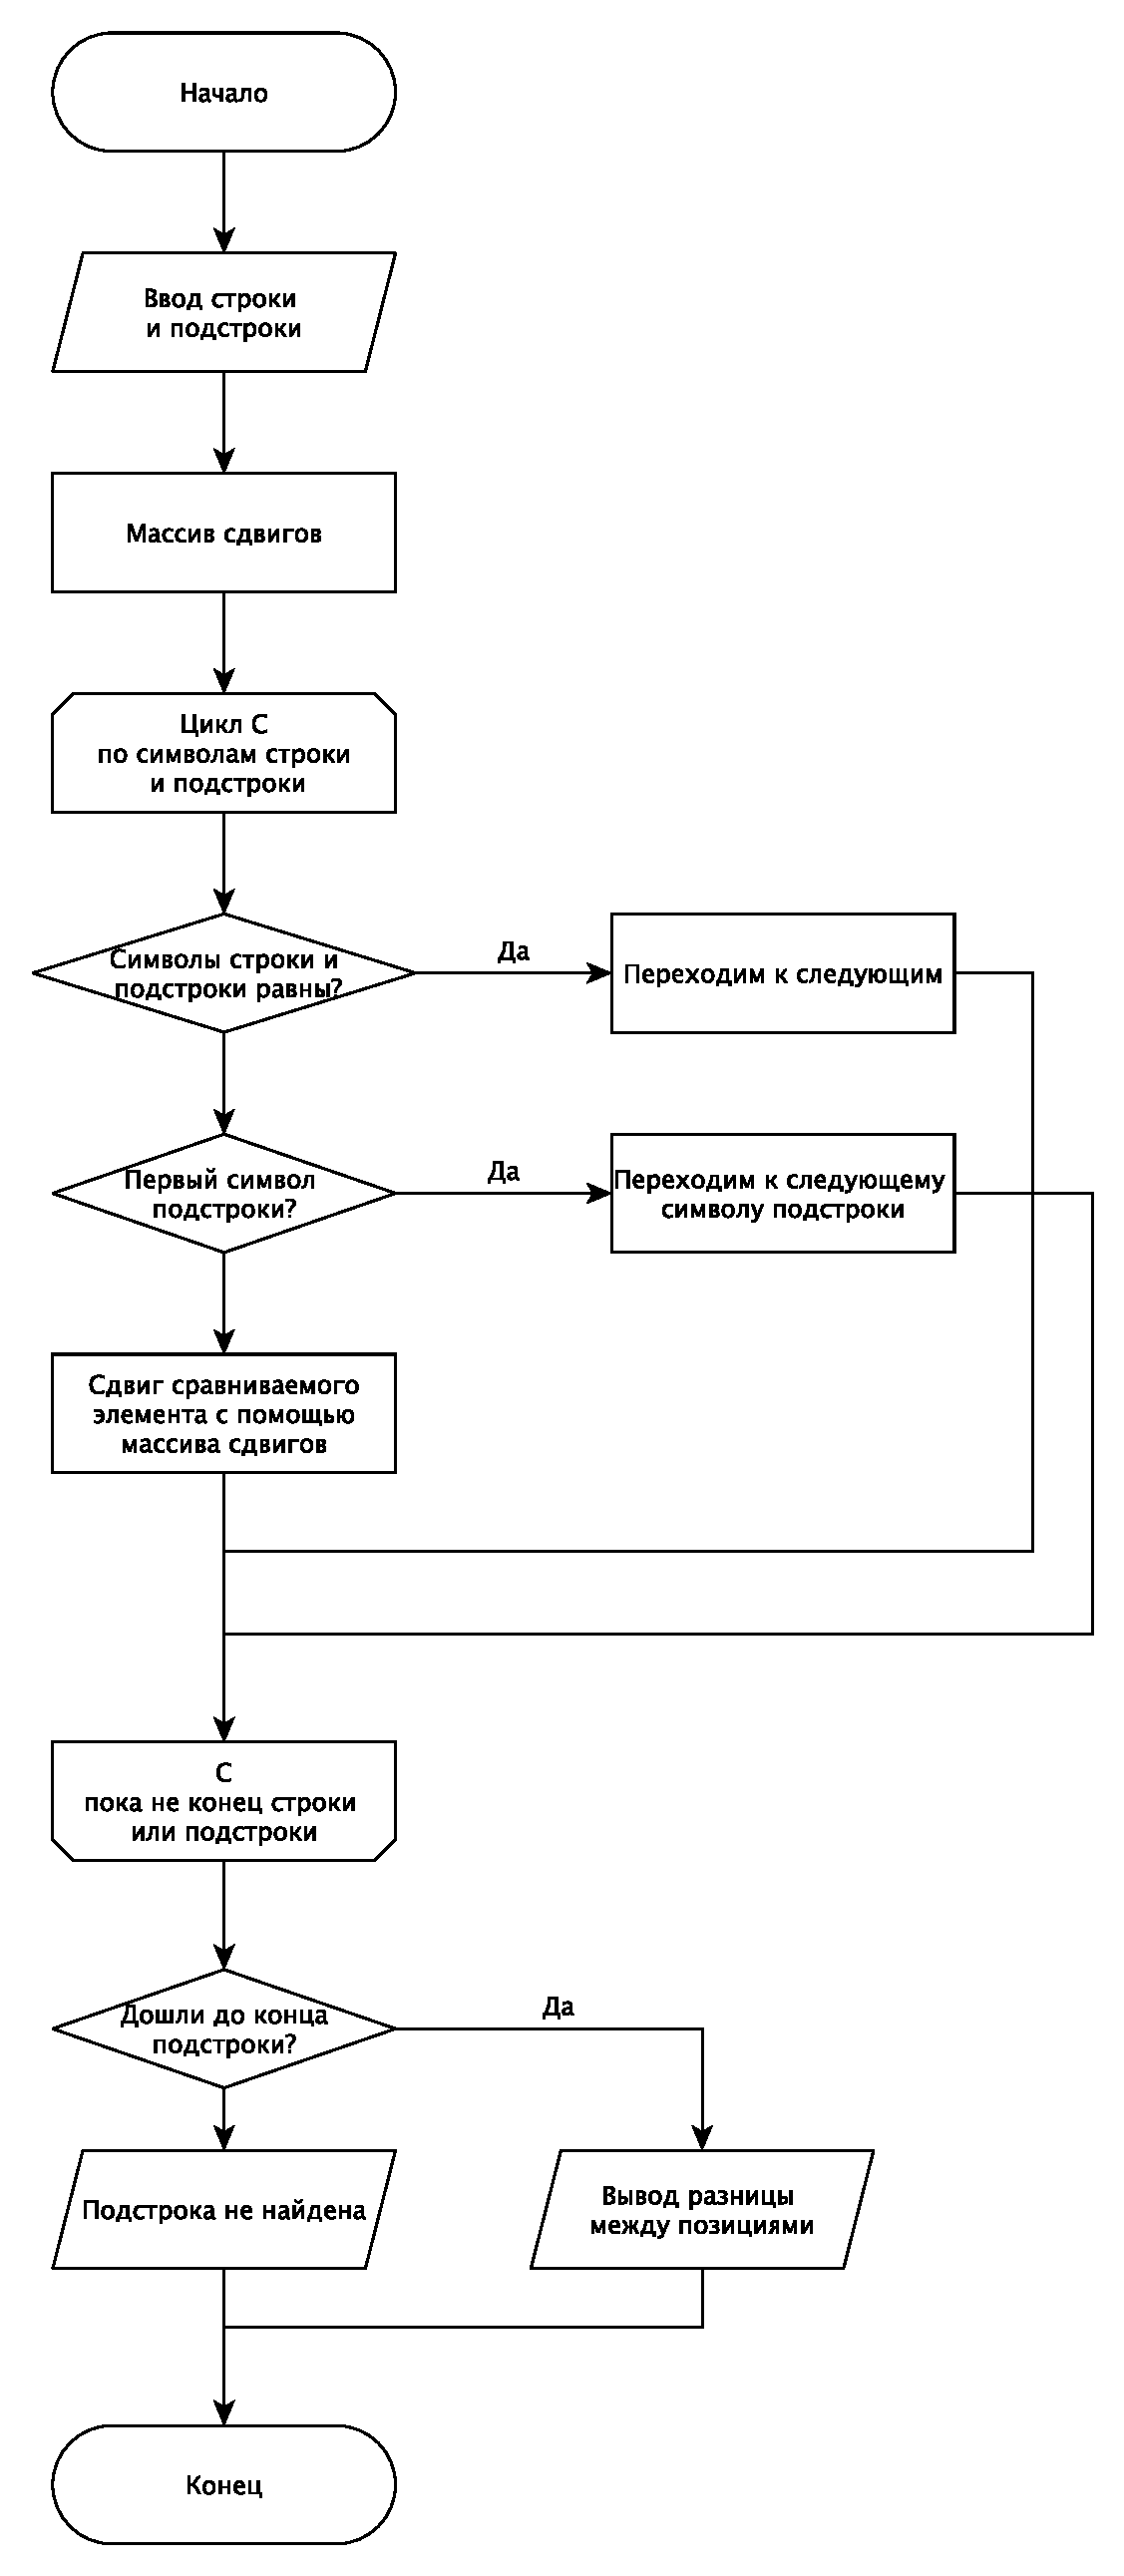
\includegraphics[scale = 0.57]{shema1} \\ Рис. 2 - Алгоритм КМП
	\end{center}
	
	\begin{center}
        		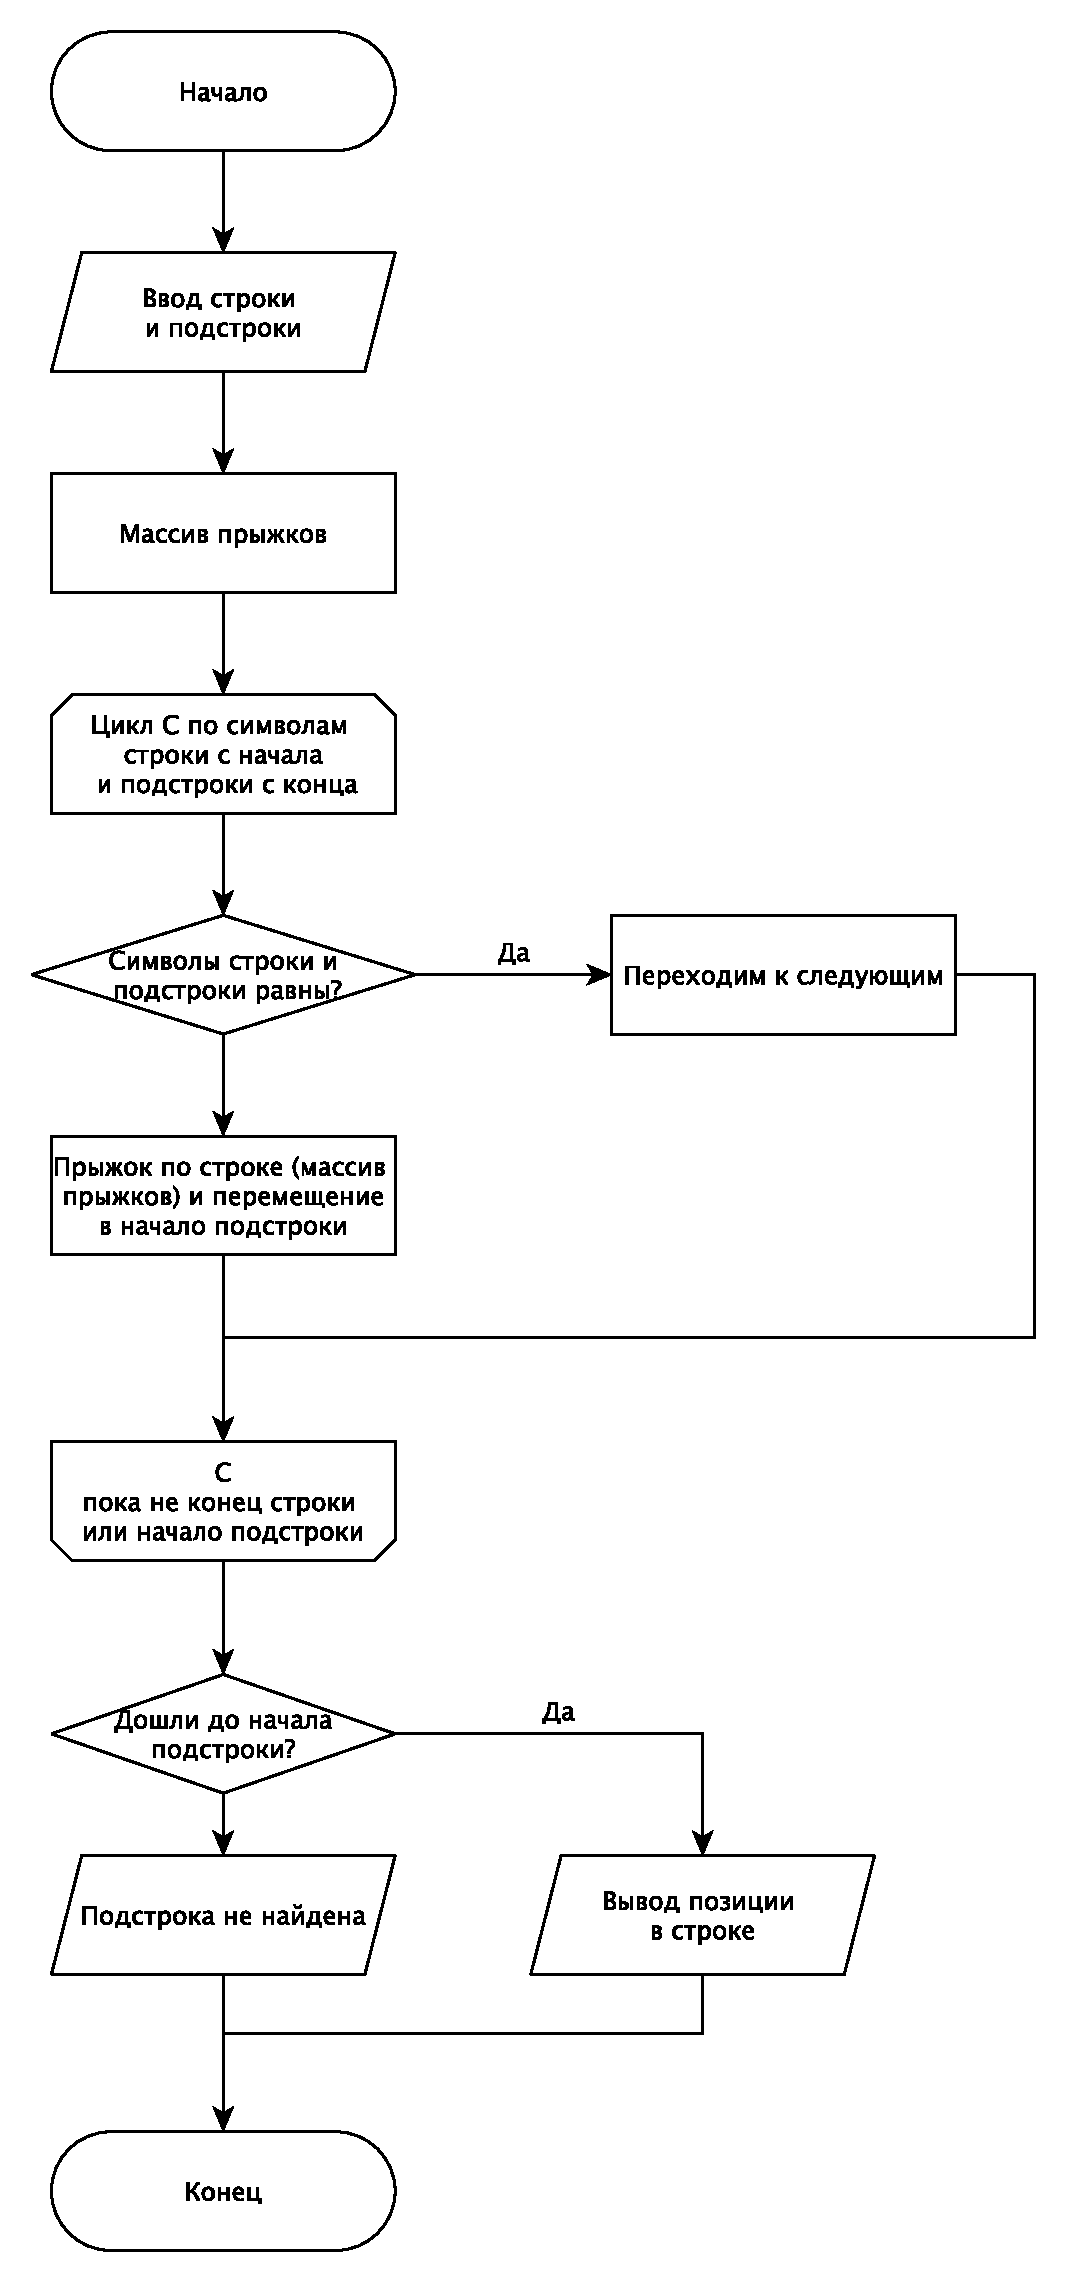
\includegraphics[scale = 0.57]{shema2} \\ Рис. 3 - Алгоритм БМ
	\end{center}
        	
	\subsection{Выводы}
	\hfill
	
	Алгоритмы изучены, необходимо приступить к реализации и тестированию. 
	
	
		
    	\newpage

        \section{Технологическая часть}
        \hfill
        
        Стоит задача реализации алгоритмов сравнения с образцом на основании автоматов, а именно Кнута - Морриса - Пратта и Бойера - Мура. 
        
        \subsection{Требования к программному обеспечению}
        \hfill
        
        ПО должно предоставлять возможность разработки и запуска программы.
        \hfill
        
        \subsection{Средства реализации}
        \hfill
        
        В качестве языка программирования был выбран С++, так как я знакома с этих языком программирования и он удовлетворяет требованиям. 
        
        \subsection{Листинг кода}
        \hfill
        
        На листингах 1 и 2 представлен код алгоритмов сравнения с образцом. 
             
\begin{lstlisting}[caption=Алгоритм Кнута - Морриса - Пратта (КМП)]
    d = shift_array(x)
    i = j = 0
    while i < len(s) and j < len(x):
        if x[j] == s[i]:
            i += 1
            j += 1
        elif 0 == j:
            i += 1
        else:
            j = d[j - 1]

    if j == len(x):
        return i - j + 1
    return -1
\end{lstlisting}

\begin{lstlisting}[caption=Алгоритм Бойера - Мура]
    d = shift_array(x)
    i = j = 0
    while i < len(s) and j < len(x):
        if x[j] == s[i]:
            i += 1
            j += 1
        elif 0 == j:
            i += 1
        else:
            j = d[j - 1]

    if j == len(x):
        return i - j + 1
    return -1
\end{lstlisting}

\subsection{Тестирование}
	\hfill
	
	В таблице 5 представлена заготовка данных для тестирования заданных алгоритмов. 
	\begin{center}
		\begin{tabular}{  | c | c | c | }
			\hline
			\textbf{Строка1} & \textbf{Строка2} & \textbf{Ожидаемый результат} \\ \hline
   			aaaaa&a&1 \\ \hline
			
   			aapo & po & 3 \\ \hline
			
			poaa & po & 1 \\ \hline
			
			qwerty & a & Подстрока не найдена \\ \hline
			
			popopopopo & po & 1 \\ \hline
			
		\end{tabular}
		
		\hfill
		
		Таблица 5.
		Подготовленные тестовые данные.  
	\end{center}
        
	
 	\subsection{Выводы}
	\hfill
	
	Алгоритмы были изучены и реализованы, необходимо приступить к тестированию. 
        
        \newpage
        

        \section{Экспериментальная часть}
        \hfill
        
        Необходимо протестировать полученную программу. 

        \subsection{Примеры работы}
	\hfill
	
	На рисунке 4 представлены примеры работы программы на разных входных данных.
	\begin{figure}[ht]\center
		\begin{tabular}{cc}
			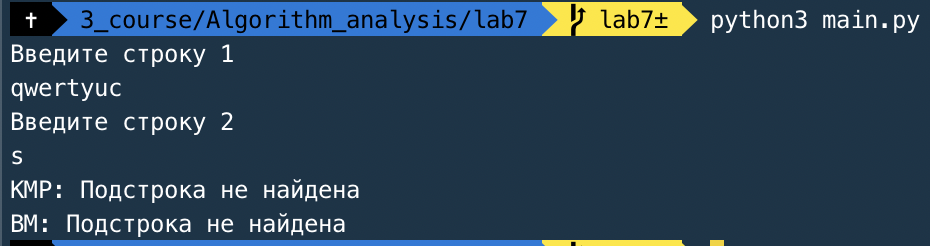
\includegraphics[width=80mm]{ex1} & 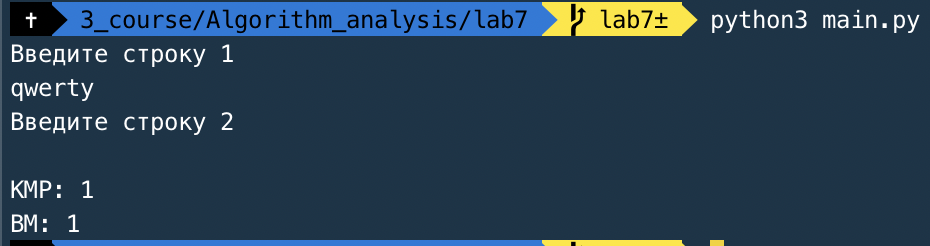
\includegraphics[width=80mm]{ex2} \\
			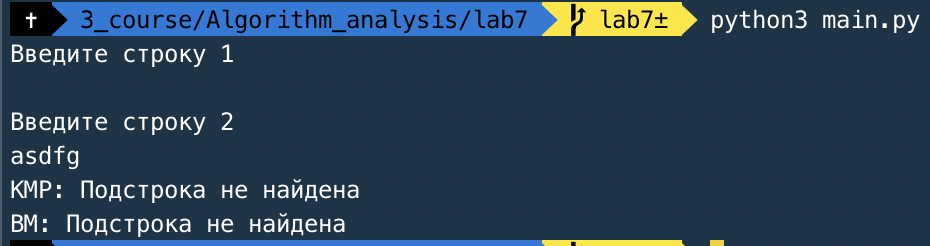
\includegraphics[width=80mm]{ex3} & 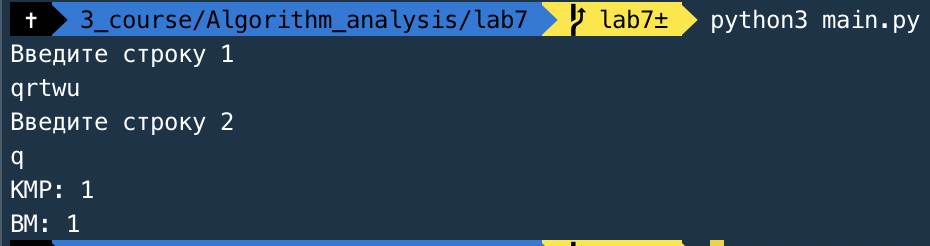
\includegraphics[width=80mm]{ex4}
		\end{tabular}
		\\ Рис. 4 - Примеры работы
	\end{figure}
	
	 \subsection{Результаты тестирования}
        
	\hfill
	Проверяем нашу программу на тестах из таблицы 5. Полученные результаты представлены в таблице 6. 
	
	\begin{center}
		\begin{tabular}{  | c | c | c | c |}
			\hline
			\textbf{Строка1} & \textbf{Строка2} & \textbf{КМП} & \textbf{БМ}  \\ \hline
   			aaaaa&a&1&1 \\ \hline
			
   			aapo & po & 3&3 \\ \hline
			
			poaa & po & 1&1 \\ \hline
			
			qwerty & a & Подстрока не найдена& Подстрока не найдена  \\ \hline
			
			popopopopo & po & 1&1 \\ \hline
			
		\end{tabular}
		
		\hfill
		
		Таблица 6.
		Тестирование программы.  
	\end{center}
	
	\textbf{Тесты пройдены}

	
	\subsection{Выводы}
	\hfill
	
	Изучены, реализованы и протестированы алгоритмы сравнения с образцом на основании автоматов. 
	
	\newpage

        \anonsection{Заключение}
        \hfill
        
        В данной работе изучены, разработаны и протестированы алгоритм поиска подстроки в строке, такие как Кнута-Морриса-Пратта и Бойера-Мура. 
        
        \hfill
	
	\textbf{Решены следующие задачи. }
	\begin{enumerate}
	\item Изучены основные алгоритмы, решающих задачу поиска. 
	\item Реализованы необходимые алгоритмы. 
	\end{enumerate}
        
       
 	\newpage

        \begin{thebibliography}{}
        
        \bibitem{} [Электронный ресурс]. - Режим доступа: https://support.office.com/ru-ru/article/Поиск-текста-в-документе-672d56af-7ad9-4b98-872c-ceed9c81c21c (дата обращения: 13.12.2019)
        
        \bibitem{} [Электронный ресурс]. - Режим доступа: https://pythonworld.ru/tipy-dannyx-v-python/stroki-funkcii-i-metody-strok.html (дата обращения: 13.12.2019)
        
         \bibitem{} Семинары
 
	\end{thebibliography} 

\end{document}
